\section{Density Estimation}
Goal: Estimate unobservable underlying probability density from observed data.\\\\
Note, probability = area under density fn curve. Integrating entire curve gives 1.\\
\subsection*{Approaches for Density Estimation}
- Parametric density estimation\\
- Nonparametric density estimation\\
\subsection*{General Principle}
Observed data points assumed to be sample of N random variables \textbf{independent 
and identically distributed (i.i.d.)}\\
\underline{Identically Distributed}: For any $x_i \in D$, it is sampled from 
sampled from same probability distribution\\
\underline{Independent}: all data points $x_i \in D$ are independent events.

\subsection*{Parametric Density Estimation}
Assume that data are drawn from known probability density family, $p(\mathbf{x}; \theta)$,
defined up to parameters, $\theta$.\\
Task: Find parameter $\theta$ that makes sampling $x_i$ from $p(\mathbf{x}; \theta)$
as likely as possible.\\\\
Approach: \textbf{Maximum Likelihood Estimation}
\subsection*{Maximum Likelihood Estimation}
Likelihood of parameter $\theta$ given sample $\mathcal{D}$: $l(\theta|\mathcal{D}) \triangleq p(\mathcal{D};\theta)$\\
Since data are i.i.d, the likelihood is product of likelihoods of individual data points:\\
\[l(\theta|\mathcal{D}) \triangleq p(\mathcal{D};\theta) = \prod^N_{i=1}p(x_i; \theta)\]
Therefore, find $\theta$ that makes $\mathcal{D}$ most likely to be drawn:
\[\hat{\theta} = \argmax_\theta l(\theta|\mathcal{D})\]
Typically, log-likelihood is used such that product can be converted into sum\\
\[ln\ l(\theta|\mathcal{D}) = \sum^N_{i=1}ln\ p(x_i; \theta)\]
\subsection*{Univariate Gaussian}
\[\mathbf{x}_i \thicksim p(\mathbf{x};\mu, \sigma^2) = \frac{1}{\sqrt{2\pi \sigma^2}}e^{(-\frac{(x-\mu)^2}{2\sigma^2})}\]
Solutions to parameters $\mu$ and $\sigma^2$ (Unbiased estimation):\\
\[\begin{cases}
    \hat{\mu} = \frac{1}{N}\sum^N_{i=1}\mathbf{x}_i \\\\
    \hat{\sigma^2} = \frac{1}{N-1}\sum^N_{i=1}(\mathbf{x}_i - \hat{\mu})^2 
\end{cases}\]
\subsection*{Multivariate Gaussian}
Solutions to parameters $\mu$ (d-dimensional mean vector)\\
and $\Sigma$ (d x d covariance matrix) (Unbiased estimation):\\

\[\begin{cases}
    \hat{\mathbf{\mu}} = \frac{1}{N}\sum^N_{i=1}\mathbf{x}_i \\\\
    \hat{\mathbf{\Sigma}} = \frac{1}{N-1}\sum^N_{i=1}(\mathbf{x}_i - \hat{\mathbf{\mu}})(\mathbf{x}_i - \hat{\mathbf{\mu}})^T
\end{cases}\]

\subsection*{Nonparametric density estimation}
\subsection*{Histogram Estimator}
\[\hat{p}(\mathbf{x})=\frac{\# x_i \text{ in same bin as } x}{N\Delta}\]
First bin start from 0, therefore determine which bin to use by using x
\subsection*{Na\"ive Estimator}
\[\hat{p}(\mathbf{x})=\frac{1}{N\Delta}\sum^N_{i=1}w(\frac{\mathbf{x} - \mathbf{x}_i}{\Delta})\]
Windowing function
\[w(u) = \begin{cases}
    1 \text{ if } -\frac{1}{2} \leq u < \frac{1}{2}\\
    0 \text{ otherwise}
\end{cases}\]

\subsection*{Generalisation to Multivariate}
If the data is d-dimensional, the bins become a d-dimensional hypercube with volume: $V=h^d$, where h is the length of each edge 
and d is the number of dimensions.

Windowing function:\\
\[w(u) = \begin{cases}
    1 \text{ if } -\frac{1}{2} \leq u_j < \frac{1}{2} \text{ for all } j \in \{1,.,d\}\\
    0 \text{ otherwise}
\end{cases}\]
\[\hat{p}(\mathbf{x})=\frac{1}{NV}\sum^N_{i=1}w(\frac{\mathbf{x} - \mathbf{x}_i}{h})\]


\subsection*{KNN Estimator}
Set the numerator as a constant (K), adapt smoothing to 
local density of data. Degree of smoothing controlled by K (number of neighbours).
\[p(\mathbf{x}) = \frac{K}{NV_x}\]
$V_x$ is the volume of the space centered at $\mathbf{x}$ that exactly contains K nearest 
neighbors of $\mathbf{x}$.\\\\

With a predefined K, for a data point $\mathbf{x}$,\\
1) Compute distance of all points to x (e.g. euclidean dist)\\
2) Sort observed data points based on distances in asc order\\
3) Obtain the k-th distance to compute $V_{d_k(\mathbf{x})}$, which is the volume 
of the d-ball\\
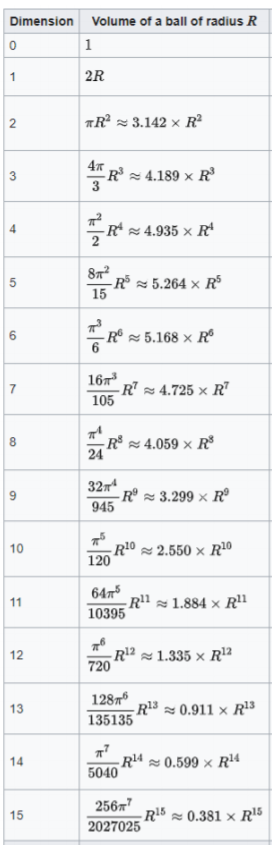
\includegraphics[width=\linewidth]{fig/knnestimator.PNG}
